\chapter{TLS-Attacker}
\section{Descrizione}

Il tool TLS-Attacker fornisce il testing di server web che implementano il protocollo TLS. E' basato su Java per analizzare le librerie TLS ed è in grado di inviare messaggi di protocollo arbitrari in un ordine arbitrario al peer TLS. Ciò offre l'opportunità di definire un flusso di protocollo TLS personalizzato e testarlo verso una libreria TLS, osservando il comportamento del server.
Transport Layer Security è un protocollo crittografico sviluppato intorno al 1999, partendo dal SSL ,oggi deprecato, che fornisce sicurezza end-to-end dei dati inviati tra applicazioni su Internet. E’ facilmente identificato anche dall’utente grazie all'icona del lucchetto che appare nei browser web quando viene stabilita una sessione sicura. Oltre ad essere implementato a livello Transport per garantire sicurezza al livello applicazione, può essere utilizzato anche per offrire sicurezza a UDP,DCCP e SCTP, dove prende il nome di DTLS ossia Data Transport Layer Security.
Il fuzzing con TLS-Attacker implica l'invio di input non corretti o imprevisti ad un'implementazione TLS per identificare vulnerabilità o punti deboli nel modo in cui gestisce i messaggi del protocollo TLS. Ciò può aiutare a identificare problemi di sicurezza come buffer overflow, perdite di memoria o altre vulnerabilità che potrebbero essere sfruttate da hacker.
\FloatBarrier
\begin{figure}[h]
    \centering
    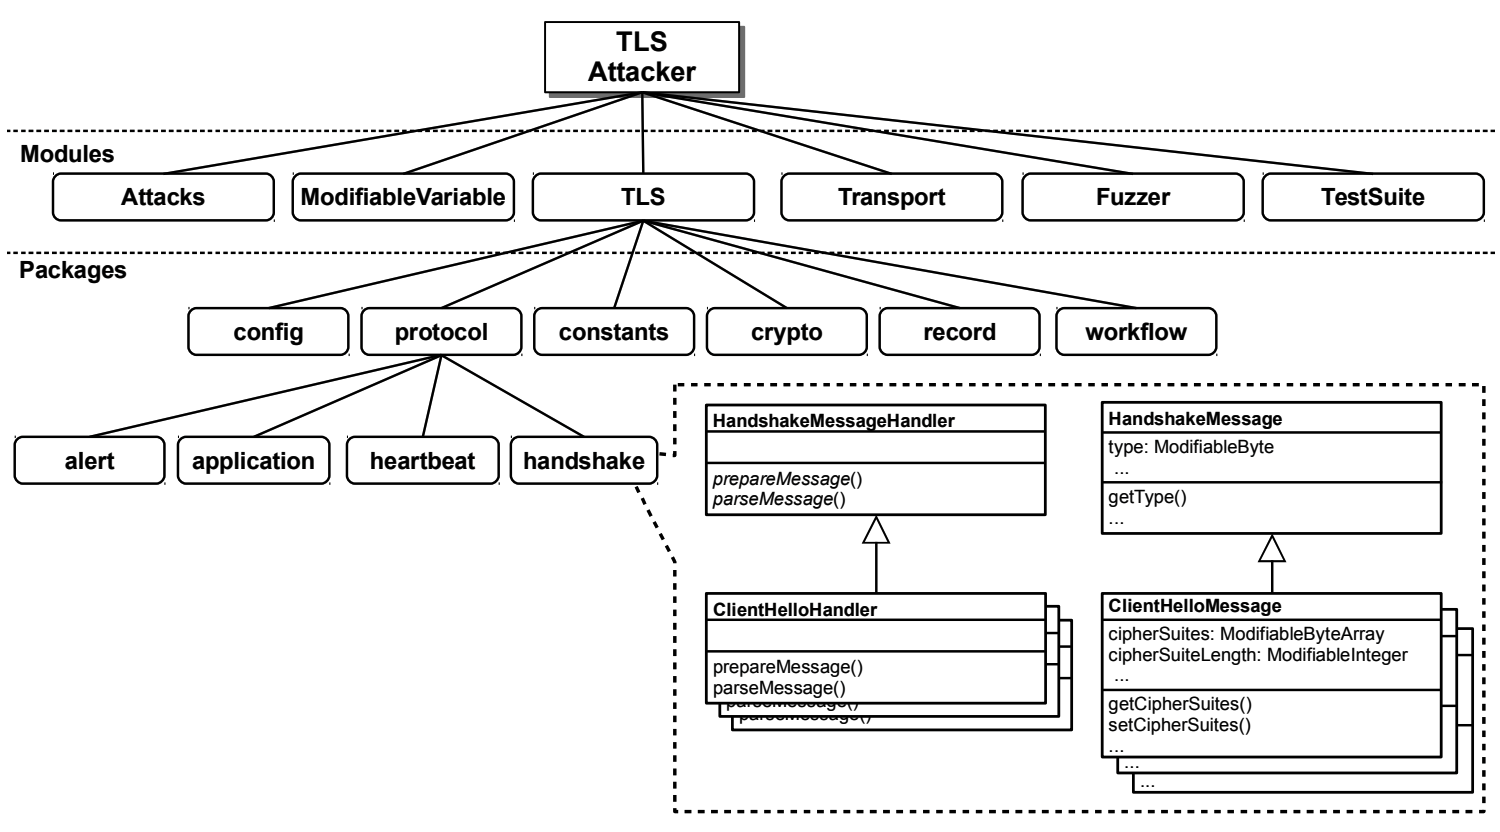
\includegraphics[width = 1.1\textwidth]{images/struttura-tls-attcaker-alto-livello.png}
    \caption{Struttura ad alto livello di TLS-Attacker.}
    \label{fig:enter-label}
\end{figure}
\FloatBarrier
\section{Handshake in TLS}
Nel protoclollo TLS vengono utilizzate le suite di cifratura, ossia un insieme di algoritmi utilizzati per rendere sicuri i collegamenti di rete basati sul medesimo protocollo. L'insieme di algoritmi che costituisce una suite comprende tipicamente: $\\$$\\$
 - \textbf{Un algoritmo per lo scambio delle chiavi crittografiche} che viene utilizzato per assicurare lo scambio corretto delle chiavi utilizzate dall'algoritmo stesso per la comunicazione tra due dispositivi.  $\\$$\\$
 - \textbf{Un algoritmo di crittografia} che esegue l'operazione di criptare e decriptare i messaggi e i dati scambiati tra le macchine comunicanti.$\\$$\\$
 - \textbf{Un algoritmo di message authentication code (MAC)}che realizza i controlli di integrità dei dati per assicurare che il messaggio non abbia subito modifiche durante la trasmissione. $\\$
 Esempio di chiave di cifratura: \textit{TLS\_RSA\_WITH\_3DES\_EDE\_CBC\_SHA256} $\\$ nella quale,$\\$
- \textbf{TLS} definisce il protocollo a cui la suite è destinata; in questo caso si tratta di TLS. $\\$
- \textbf{RSA} indica l'algoritmo di scambio delle chiavi utilizzato. Questo algoritmo si usa per determinare se e in che modo il client e il server si autenticano reciprocamente durante l'handshake. $\\$
- \textbf{3DES\_EDE\_CBC} indica il tipo e la modalità della cifratura a blocchi usata per codificare il flusso di messaggi. $\\$
- \textbf{SHA256} indica l'algoritmo di message authentication code usato per garantire l'integrità e l'autenticità del messaggio, basato su una chiave a 256 bit. $\\$
\begin{figure}[h]
    \centering
    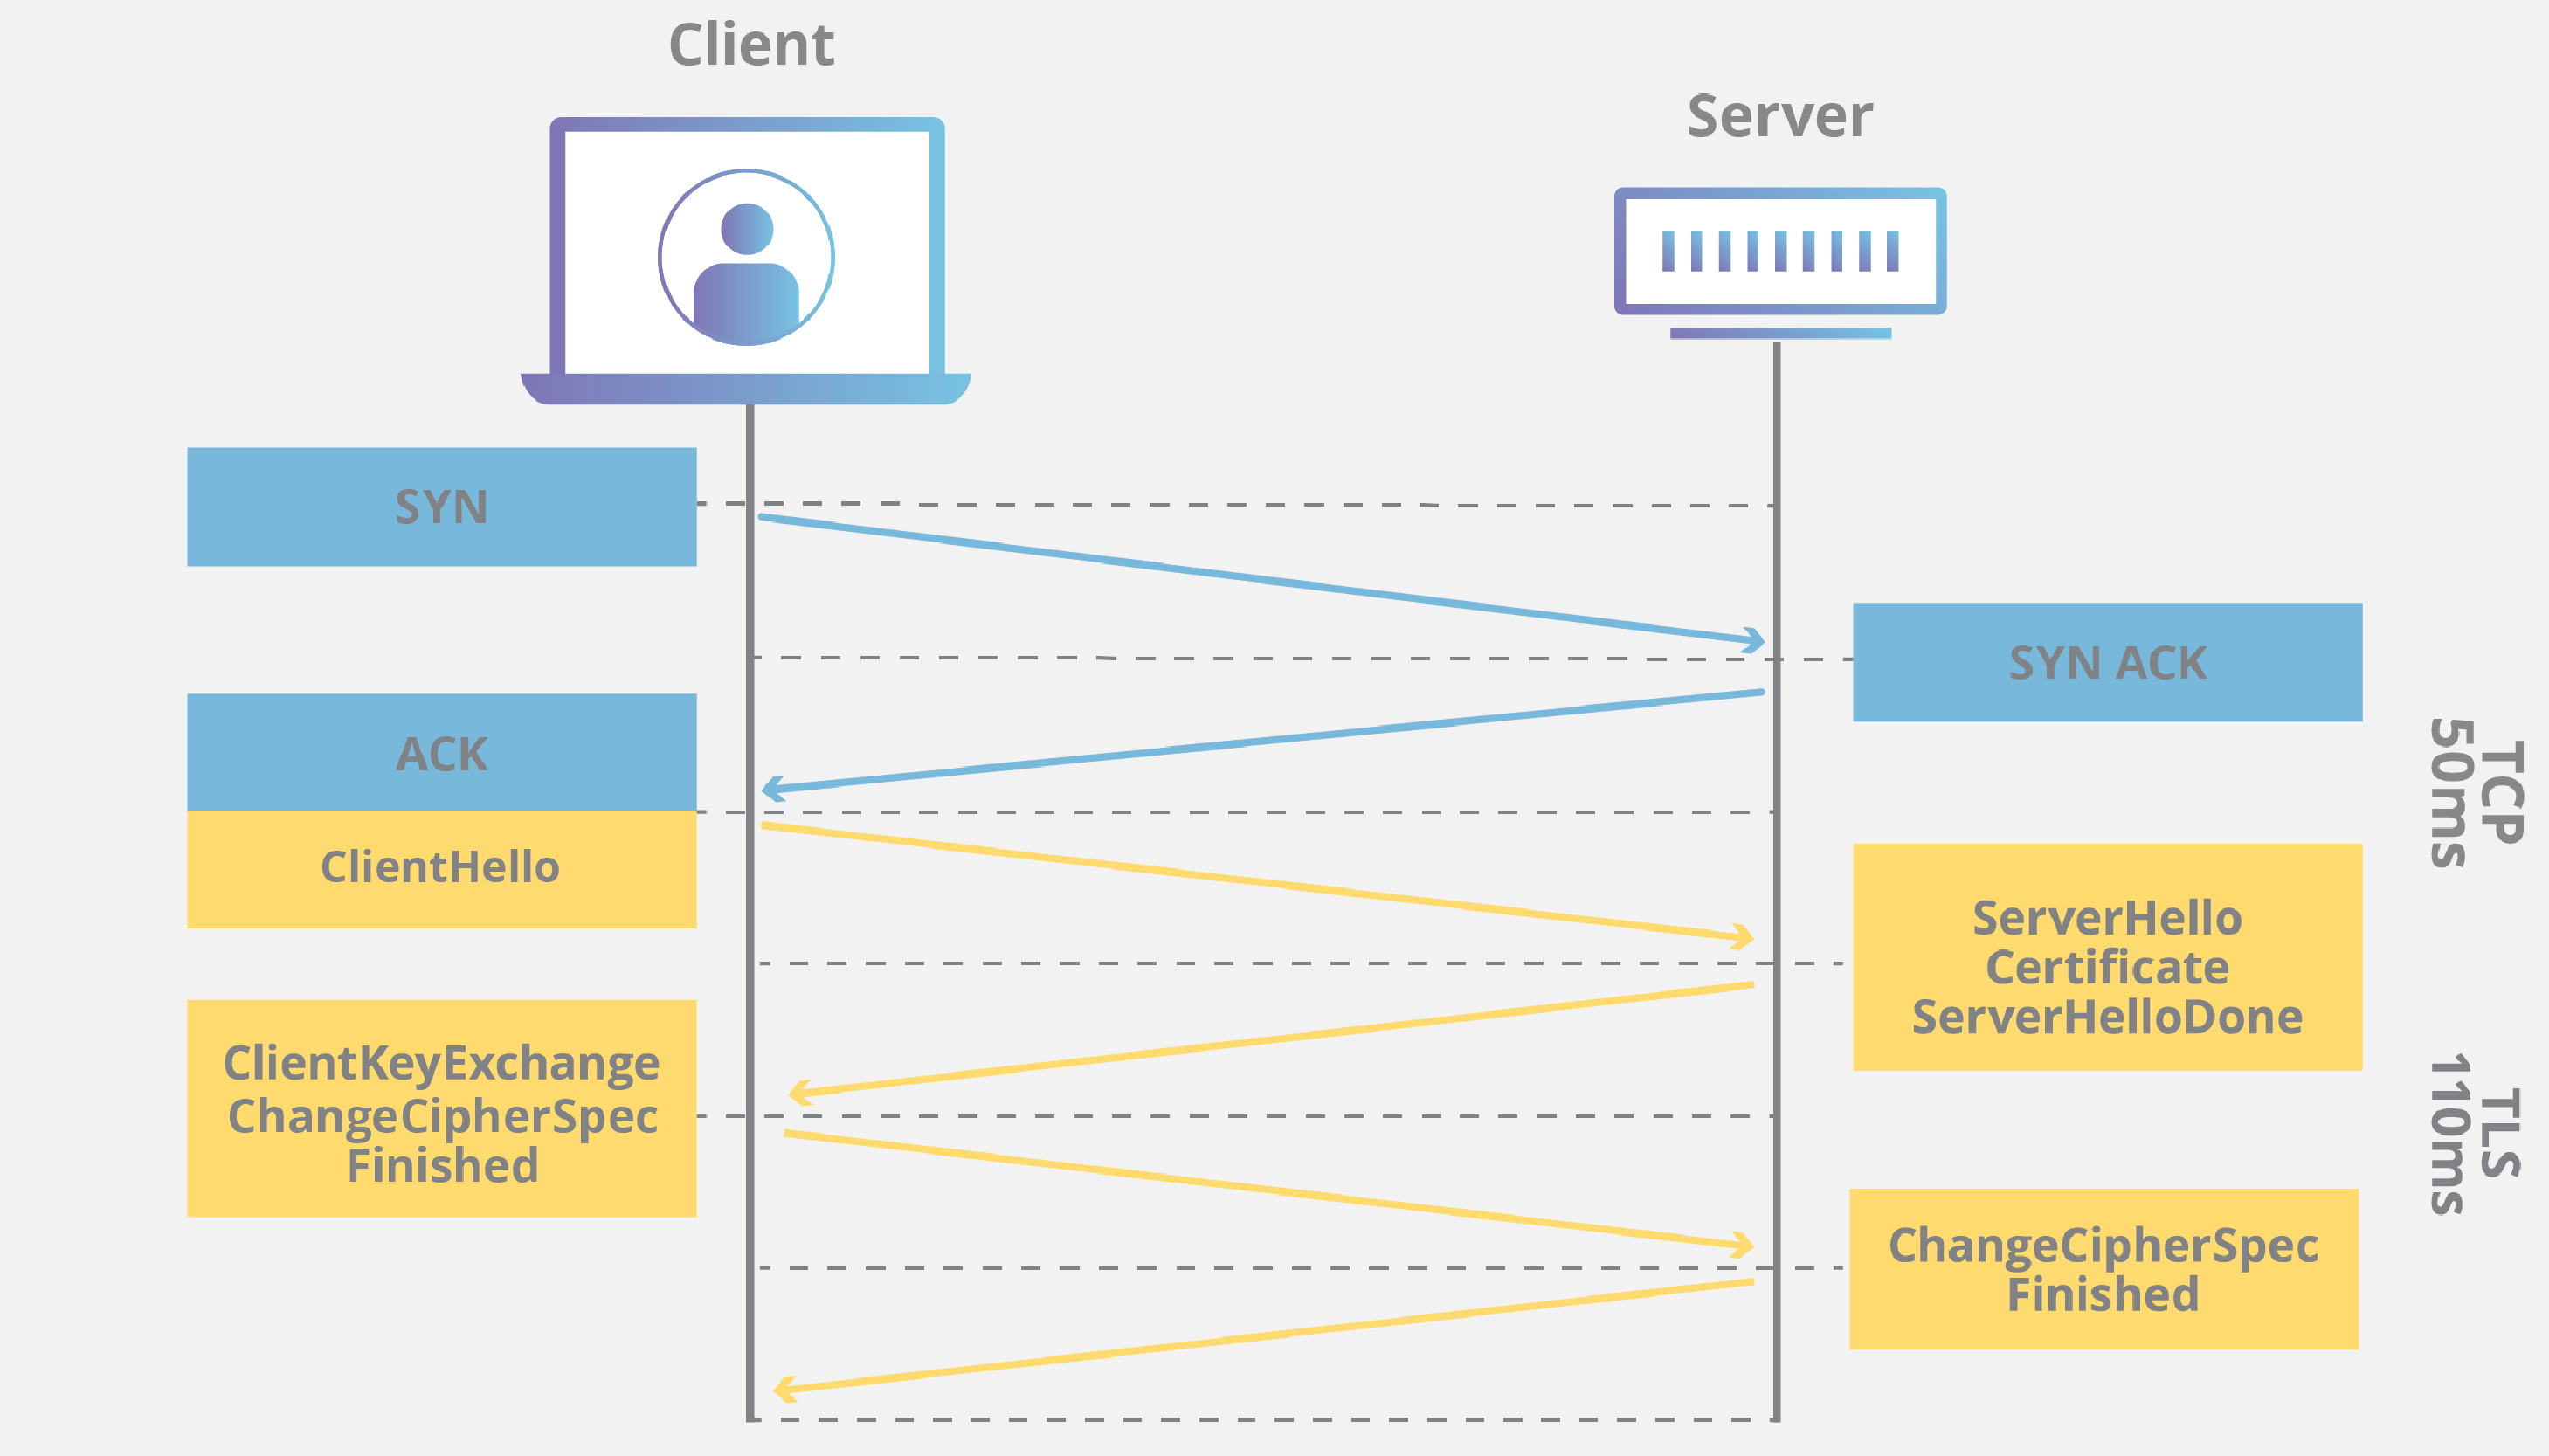
\includegraphics[width = 1.0\textwidth]{images/tls-handshake.png}
    \caption{Handshake nel protocollo TLS.}
    \label{fig:enter-label}
\end{figure}
\FloatBarrier

$\\$
Il funzionamento dell'handshake TLS quindi si basa fondamentalmente sullo scambio di alcuni messaggi tra client e server per stabilire una connessione sicura. Il client invia un messaggio "Client hello" al server, insieme al valore casuale del client e ai pacchetti di crittografia supportati.
Il server risponde inviando un messaggio "Server hello" al client, insieme al valore casuale del server. Il server quindi invia il certificato al client per l'autenticazione e può richiedere un certificato dal client. Il server invia anche il messaggio "Server hello done", il quale conferma il completamento della prima fase dell'handshake. Se il server ha richiesto un certificato dal client, il client lo invia. Il client crea ora un segreto pre-master casuale e lo crittografa con la chiave pubblica dal certificato del server, inviando il segreto pre-master crittografato al server. Il server riceve quindi il segreto pre-master. Successivamente il server e il client generano le chiavi master secret e sessione in base al segreto pre-master precedentemente scambiato. Il client invia una notifica "Modifica spec di crittografia" al server per indicare che il client inizierà a usare le nuove chiavi di sessione per l'hashing e la crittografia dei messaggi. Il client invia anche un messaggio "Client completato". Il server riceve "Cambia spec di crittografia" e commuta lo stato di sicurezza del livello record alla crittografia simmetrica usando le chiavi di sessione. Il server invia un messaggio "Server completato" al client. Il client e il server possono ora scambiare i dati dell'applicazione tramite il canale protetto stabilito. Tutti i messaggi inviati dal client al server e dal server al client vengono crittografati usando la chiave di sessione.


\section{Struttura del tool}
TLS-Attacker è implementato in linguaggio Java e supportato da alcuni progetti Maven: $\\$ $\\$
\textbf{TLS-Client}: Applicazione client $\\$
\textbf{TLS-Core}: Stack di protocollo e nucleo del tool $\\$
\textbf{TLS-Mitm}: Prototipo attacco Man In The Middle $\\$
\textbf{TLS-Server}: Applicazione server $\\$
\textbf{TLS-Proxy}: TLS-Attacker per SSLSockets $\\$
\textbf{TraceTool}: Modifiche del workflow di TLS-Attacker $\\$
\textbf{Transport}: Funzioni per livello Transport $\\$
\textbf{Utils}: Altre funzioni $\\$ 
$\\$
Il cuore del framework è l'implementazione di un costrutto
chiamato \textbf{ModifiableVariable}. Essa consente di impostare modifiche ai tipi di dati semplici, come gli interi o gli array di byte, prima o dopo che i loro valori vengano effettivamente determinati. Una \textbf{ModifiableVariable} contiene il valore originale di una specifica variabile
e fornisce il suo valore con un metodo getter. Durante l'accesso alla
alla variabile, \textbf{ModifiableVariable} è in grado di applicare modifiche predefinite. $\\$
Tutti i messaggi di protocollo, ad esempio durante l'handshake descritto in precedenza, vengono salvati in questa variabile. $\\$ $\\$
Esempio di codice per un messaggio ClientHello dove vengono utilizzate le \textbf{ModifiableVariable} per memorizzare i vari dati necessari per l'handshake:

\begin{verbatim}
    public class ClientHelloMessage  {
      ModifiableInteger compressionLength;  
      ModifiableByteArray compression;
      ModifiableInteger chipherSuiteLenght;
      ModifiableByteArray chipherSuites;
      ...
     }
\end{verbatim}
$\\$
Prima di eseguire il protocollo, le \textbf{ModifiableVariable} permettono di impostare modifiche arbitrarie alle variabili o di definire valori espliciti delle variabili. Le variabili vengono poi modificate dinamicamente durante l'esecuzione del protocollo. Per esempio, lo sviluppatore può utilizzare 2 suite di cifratura e impostare il valore esplicito di cipherSuitesLength a 5. TLS-Attacker utilizza quindi un valore di lunghezza non valido durante la serializzazione del messaggio ClientHello, il quale potrebbe causare un overflow. $\\$ $\\$
Il tool contiene poi altri package, come il package \textbf{Protocol}, che contiene i messaggi di protocollo e il package \textbf{Workflow}, il quale contiene l'implementazione, flessibile, del flusso di protocollo che consente di definire arbitrariamente l'ordine dei messaggi. In particolare il package \textbf{Protocol} implementa i messaggi di protocollo TLS e i loro gestori (\textbf{handler}). Ogni messaggio di protocollo è definito da un \textbf{handler} (responsabile dell'elaborazione del messaggio) e da uno stato del messaggio (che rappresenta lo stato attuale del messaggio TLS). Ad esempio, il pacchetto handshake contiene le classi HandshakeMessageHandler e HandshakeMessage (vedi Figura 1.1). Il package \textbf{Workflow} contiene  l'esecuzione del protocollo TLS. L'esecuzione del protocollo TLS dipende esclusivamente dai messaggi TLS predefiniti (comunque modificabili arbitrariamente). 


\section{Utilizzo}
Durante il mio studio ed utilizzo di TLS-Attacker sono stati fatti diversi test di server TLS per analizzare il comportamento del tool e dei server stessi. Il primo tipo di test effettuato si basa sulle modifiche del \textbf{WorkflowTrace} per poter trovare vulnerabilità all'attacco Bleichenbacher, il quale si basa sullo scovare il \textbf{premaster secret}. I server testati sono stati aperti direttamente sul mio PC grazie ad una funzionalità apposita presente in TLS-Attacker. Il seguente codice permette di testare le contromisure verso un attacco Bleichenbacher:

{\footnotesize 
\begin{verbatim} 
    TlsContext context = initializeTlsContext (config);
    WorkflowExecutor executor = initializeWorkflowExecutor(context);

    //modifica esplicita del premaster secret
    RSAClientKeyExchangeMessage rsa = new RSAClientKeyExchangeMessage();
    ModifiableVariable<byte[]> = pms = new ModifiableVariable<>();
    pms.setMOdification( new explicitValueModification (VALUE));
    pms.setPlaidPannedPremasterSecret(pms);

    //flusso del messaggio di protocollo
    List<ProtocolMessage> m = context.getProtocolMessages();
    m.add(new ClientHelloMessage());
    m.add(new ServerHelloMessage());
    m.add(new CertificateMessage());
    m.add(new ServerHelloDoneMessage());
    m.add(rsa);
    m.add(new ChangeChipherSpecMessage(ConnectionEnd.CLIENT));
    m.add(new FinishedMessage(ConnectionEnd.CLIENT));
    m.add(new Alert(ConnectionEnd.SERVER));

    //esecuzione del protocollo
    executor.executeWorkflow();
\end{verbatim}
}
$\\$
Impostando un premaster secret personalizzato, si va a forzare l'utilizzo di TLS-Attacker con questo valore. $\\$
Apertura del server di test: \textit{openssl s\_server -key rsa1024\_key.pem -cert rsa1024\_cert.pem}
Quì, i file RSA indicano l’algoritmo di scambio delle chiavi utilizzato ed in particolare come il client ed il server si autenticano reciprocamente durante l’handshake.  Il client TLS esegue un handshake per la suite di crittografia selezionata. $\\$
Connessione al server di test: \textit{java -jar TLS-Client.jar -connect localhost:4433} $\\$
\begin{figure}[h]
    \centering
    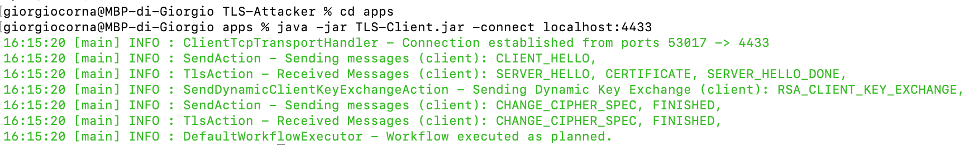
\includegraphics[width = 1.1\textwidth]{images/test-server1.png}
    \caption{Risultato handshake di connessione al server aperto.}
    \label{fig:enter-label}
\end{figure}
\FloatBarrier
$\\$
Inoltre è possibile tenere traccia dei valori che vengono effettivamente scambiati durante l’esecuzone del WorkflowTrace. Per fare ciò TLS-Attacker può salvare tutto in un file tramite il parametro \textit{-workflow\_output ‘nomefile’.xml}
Si può anche specificare l’utilizzo di una specifica suite di crittografia: \textit{java -jar TLS-Client.jar -connect localhost:4433 -cipher TLS\_RSA\_WITH\_AES\_256\_CBC\_SHA -version TLS11}
E' possibile creare \textbf{WorkflowTrace} personalizzati anche in linguaggio XML: 
{\footnotesize 
\begin{verbatim}
    <workflowTrace>
    <Wait>
         <time>5000</time>
    </Wait>
    <Send>
        <messages>
            <ServerHello/>
        </messages>
    </Send>
    <Receive>
        <expectedMessages>
            <ClientHello/>
            <Certificate/>
            <ServerHelloDone/>
        </expectedMessages>
    </Receive>
</workflowTrace>
\end{verbatim}
}
$\\$
Il caso quì testato, correttamente, ritorna un errore: $\\$
\begin{figure}[h]
    \centering
    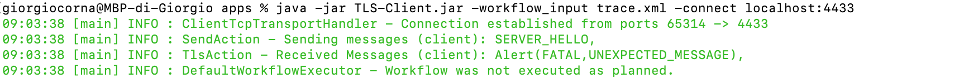
\includegraphics[width = 1.1\textwidth]{images/test-server2.png}
    \caption{Risultato handshake di connessione con errore al server aperto.}
    \label{fig:enter-label}
\end{figure}
\FloatBarrier
$\\$
Il protocollo TLS infatti prevede un handshake con un workflow ben preciso, come descritto nella \textbf{figura 1.2}. Nel caso testato invece viene inviato al server come primo messaggio un 'ServerHello'. Il server, di conseguenza, risponde correttamente con un messaggio d'errore come descritto nella \textbf{figura 1.4}, avvertendo della ricezione di un messaggio inaspettato. $\\$
Un altra tipologia di test consiste nell'effetturare la verifica della corretta suite di crittografia scelta. Nel file Config di default viene specificato l’utilizzo di una suite di crittografia di tipo RSA, per tanto se provassimo un handshake verso server che non utilizzano quel tipo di crittografia, otterremmo un errore. $\\$
Tramite il parametro -cipher ‘nomesuite’ possiamo forzare l’utilizzo di una determinata suite di crittografia. Quindi tra client e server, durante l’handshake, vengono condivise tutte le suite di crittografia utilizzabili, mentre se ne si specifica una, verrà condivisa (e quindi scelta) solo quella. 
$\\$
\begin{figure}[h]
    \centering
    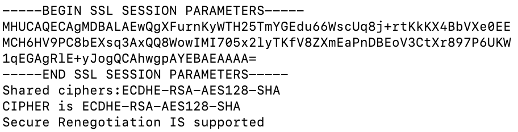
\includegraphics[width = 1.1\textwidth]{images/ssl-server-con-chipher-suite-spec.png}
    \caption{Apertura server con chipher suite specifica.}
    \label{fig:enter-label}
\end{figure}
\FloatBarrier
\begin{figure}[h]
    \centering
    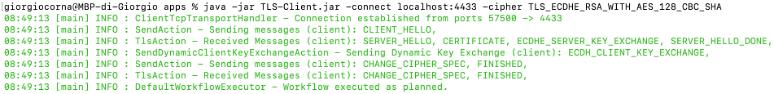
\includegraphics[width = 1.1\textwidth]{images/risultato-chipher-suite-spec.png}
    \caption{Risultato test server con chipher suite specifica.}
    \label{fig:enter-label}
\end{figure}
\FloatBarrier
\section{Fuzzing con TLS-Attacker}
TLS-Attacker è stato utilizzato anche per svolgere vero e proprio fuzzing. Un esempio è il testing del \textbf{buffer overflow}. In sostanza, si verifica \textbf{buffer overfow} quando si forniscono a un programma troppi dati. I dati in eccesso danneggiano lo spazio vicino in memoria e possono alterare altri dati. Di conseguenza, il programma potrebbe segnalare un errore o comportarsi diversamente. Tre distinte fasi costituiscono il fuzzing con TLS-Attacker per identificare vulnerabilità di questo tipo: $\\$
 - \textbf{Fase 1: Ricerca di variabili rilevanti} $\\$
Il flusso del protocollo TLS e i suoi messaggi contengono un'enorme quantità di variabili: lunghezza del messaggio, chiavi o certificati. Solo con alcune di queste variabili è possibile fare fuzzing. Per esempio alcune variabili non vengono validate dal protocollo oppure contengono valori casuali che non influenazano il comportamento del protocollo. Per tanto, esse vengono scartate per non essere utilizzate nella fase successiva.  $\\$
- \textbf{Fase 2: Fuzzing con le variabili selezionate} $\\$
Ora continuiamo quindi con le variabili scelte in precedenza. Durante questa fase sono stati eseguiti diversi test modificando casualmente delle variabili in flussi di protocollo corretti e valutando il comportamento del server. $\\$
- \textbf{Fase 3: Fuzzing con flussi di protocollo casuali} $\\$
Durante questa ultima fase vengono inviate nuovamente altre richieste al server di test utilizzando flussi di protocollo differenti. Quindi, se nella fase precedente si utilizzava un solo flusso di proocollo corretto modificandone le variabili di interesse, ora la sicurezza del server viene testata utilizzando flussi di protocollo diversi fra loro. 
$\\$ $\\$
Per esempio, proviamo a modificare il parametro, quindi una \textbf{ModifiableVariable}, che indica la versione del protocollo. Per fare ciò, modifichiamo il \textbf{WorkflowTrace} nel messaggio di ServerHello che originariamente è impostato così: $\\$
\begin{verbatim}
    <protocolVersion>
     <originalValue>03 03</originalValue>
    </protocolVersion>
\end{verbatim} $\\$
Per ragioni storiche, 0x0303 indica la versione TLS 1.2. Troviamo quindi questi tipi di variabili: $\\$
- ModifiableBigInteger: add, explicitValue, shiftLeft, shiftRight, subtract, xor $\\$
- ModifiableBoolean: explicitValue, toggle $\\$
- ModifiableByteArray: delete, duplicate, explicitValue, insert, shuffle, xor $\\$
- ModifiableInteger: add, explicitValue, shiftLeft, shiftRight, subtract, xor $\\$
- ModifiableLong: add, explicitValue, subtract, xor $\\$
- ModifiableByte: add, explicitValue, subtract, xor $\\$
- ModifiableString: explicitValue $\\$ 
Ad esempio, se vogliamo modificare un valore di lunghezza 1 Byte utilizzeremo una \textbf{ModifiableByte}, mentre se vogliamo modificare un valore di lunghezza fino a 4 Byte useremo una \textbf{ModifiableInteger}. Proviamo quindi a forzare TLS-Attacker ad inviare la versione 0x3A3A del protocollo. Siccome <ProtocolVersion> è una variabile di tipo ByteArray andremo a scrivere nel WorkflowTrace del messaggio ServerHello: $\\$
\begin{verbatim}
    <Send>
        <messages>
            <ServerHello>
                <protocolVersion>
                    <byteArrayExplicitValueModification>
                        <explicitValue>
                            3A 3A
                        </explicitValue>
                    </byteArrayExplicitValueModification>
                </protocolVersion>
            </ServerHello>
        </messages>
    </Send>
\end{verbatim} $\\$
Ora, utilizzando il comando della \textbf{figura 1.3} e specificando il workflow di input appena modificato tramite il comando \textit{-workflow\_input} si può osservare, attraverso un tool per analizzare il traffico di pacchetti come ad esempio Wireshark, che la versione del protocollo è stata cambiata. 

 
